%%%%%%%%%%%%%%%%%%%%%%%%%%%%%%%%%%%%%%%%%%%%%%%%%%%%%%%%%%%%%%%%%%%%%%%%%%%%%%%%%%%%%%%%%%%%%%%%%%%
% Chapter 2 -> Background
% Author: Mingbo Cheng
%%%%%%%%%%%%%%%%%%%%%%%%%%%%%%%%%%%%%%%%%%%%%%%%%%%%%%%%%%%%%%%%%%%%%%%%%%%%%%%%%%%%%%%%%%%%%%%%%%%
%\addbibresource{~/MEGA/MEGAsync/phd/thesis_Cheng/preamble/thesis.bib}
%\addbibresource{/home/mingbo/MEGAsync/phd/thesis_Cheng/preamble/thesis.bib}
\chapter{Background}
\label{cha:background}
\graphicspath{{chapter2/figs/}}

In this chapter, we provide a comprehensive overview of the background knowledge necessary for understanding the thesis, encompassing both biological and computational aspects. We begin by delving into molecular biology involving DNA organization, chromatin accessibility, and gene regulation~(\sref{background:DNA_Chromatin_Regulation}). Next, we explore the advancements in single-cell sequencing technologies, covering single-cell transcriptome profiling, and open chromatin measurements in single cells. This section also encompasses sequencing protocols capable of simultaneously measuring multiple types of features, known as multimodal sequencing~(\sref{background:profiling_singlecell}). Following that, we introduce computational approaches for analyzing various single-cell technology assays including single-cell RNA-seq analysis, single-cell ATAC-seq analysis, and single-cell surface protein analysis~(\sref{background:computational_singlecell}). Subsequently, we present the computational workflow for multimodal analysis. Following that, we outline two main problems that need to be addressed in single-cell multimodal analysis. The first problem is multimodal integration. For this, we first discuss the challenges associated with the task. We then introduce the current state-of-the-art methods for multimodal integration, aligning with our objective to address the issues. The second problem is trajectory inference for multimodal data. Similarly, we first present the challenge of trajectory inference. Next, we introduce the current state-of-the-art methods for trajectory inference, aligning with our goals for solving the trajectory inference issues in our method~(\sref{background:multimodal}). Finally, we conclude the chapter with a final discussion on the background~(\sref{background:Discussion}).


\section{DNA Organization, chromatin accessibility and gene regulation}
\label{background:DNA_Chromatin_Regulation}
In the symphony of life, the function of DNA organization, chromatin accessibility, and gene regulation orchestrates a harmonious dance that dictates the fate and functioning of every living organism. This dance is involved in the process in the central dogma of molecular biology~\citep{crick1970central} which describes the process by which genetic information is transferred from DNA to RNA and eventually translated to protein~(\fref{fig:central_dogma}). We start this section by first introducing DNA organization. Next, we talk about gene regulation followed by the introduction of chromatin accessibility.

\begin{figure}[!ht]
	\centering
	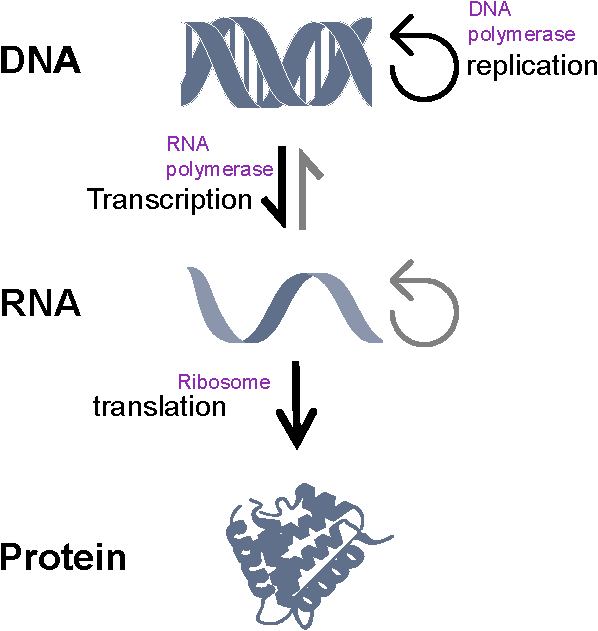
\includegraphics[width=0.65\textwidth]{central_dogma/fig}
	\vspace{0.1cm}
	\caption[central dogma.]{Central dogma of molecular biology including DNA replication, transcription and RNA translation.}
	\label{fig:central_dogma}
\end{figure}

Deoxyribonucleic Acid, or DNA is the genetic blueprint of life, containing the instructions for the development and functioning of living organisms. It is a long, double-stranded helical structure composed of four nucleotide building blocks: adenine (A), thymine (T), cytosine (C), and guanine (G). The sequence of these nucleotides forms the genetic code, encoding instructions for the development, functioning, and maintenance of all living organisms. DNA is organized into structures called chromosomes, which are located in the cell nucleus.



Gene regulation refers to the mechanisms that control the expression of genes. While an organism's DNA carries the instructions for a vast array of biological processes, not all genes are active all the time. Gene regulation allows cells to turn genes on or off, and to fine-tune their activity. This regulation is achieved through the interaction of regulatory proteins, transcription factors, and other molecules that bind to specific DNA sequences, influencing the initiation or inhibition of transcription. The transcribed RNAs next undergo a crucial process known as splicing, wherein a single pre-mRNA can give rise to various mRNAs. Following this, the resulting mRNAs are translated into proteins, and these proteins may undergo multiple post-translational modifications that can impact their activity. These modifications include ubiquitylation, methylation, phosphorylation, or acetylation~\citep{wang2014protein} (\fref{fig:central_dogma}).

%Epigenetic modifications, such as DNA methylation and histone modification, also play a crucial role in gene regulation by modifying the accessibility of DNA.

\begin{figure}[!ht]
	\centering
	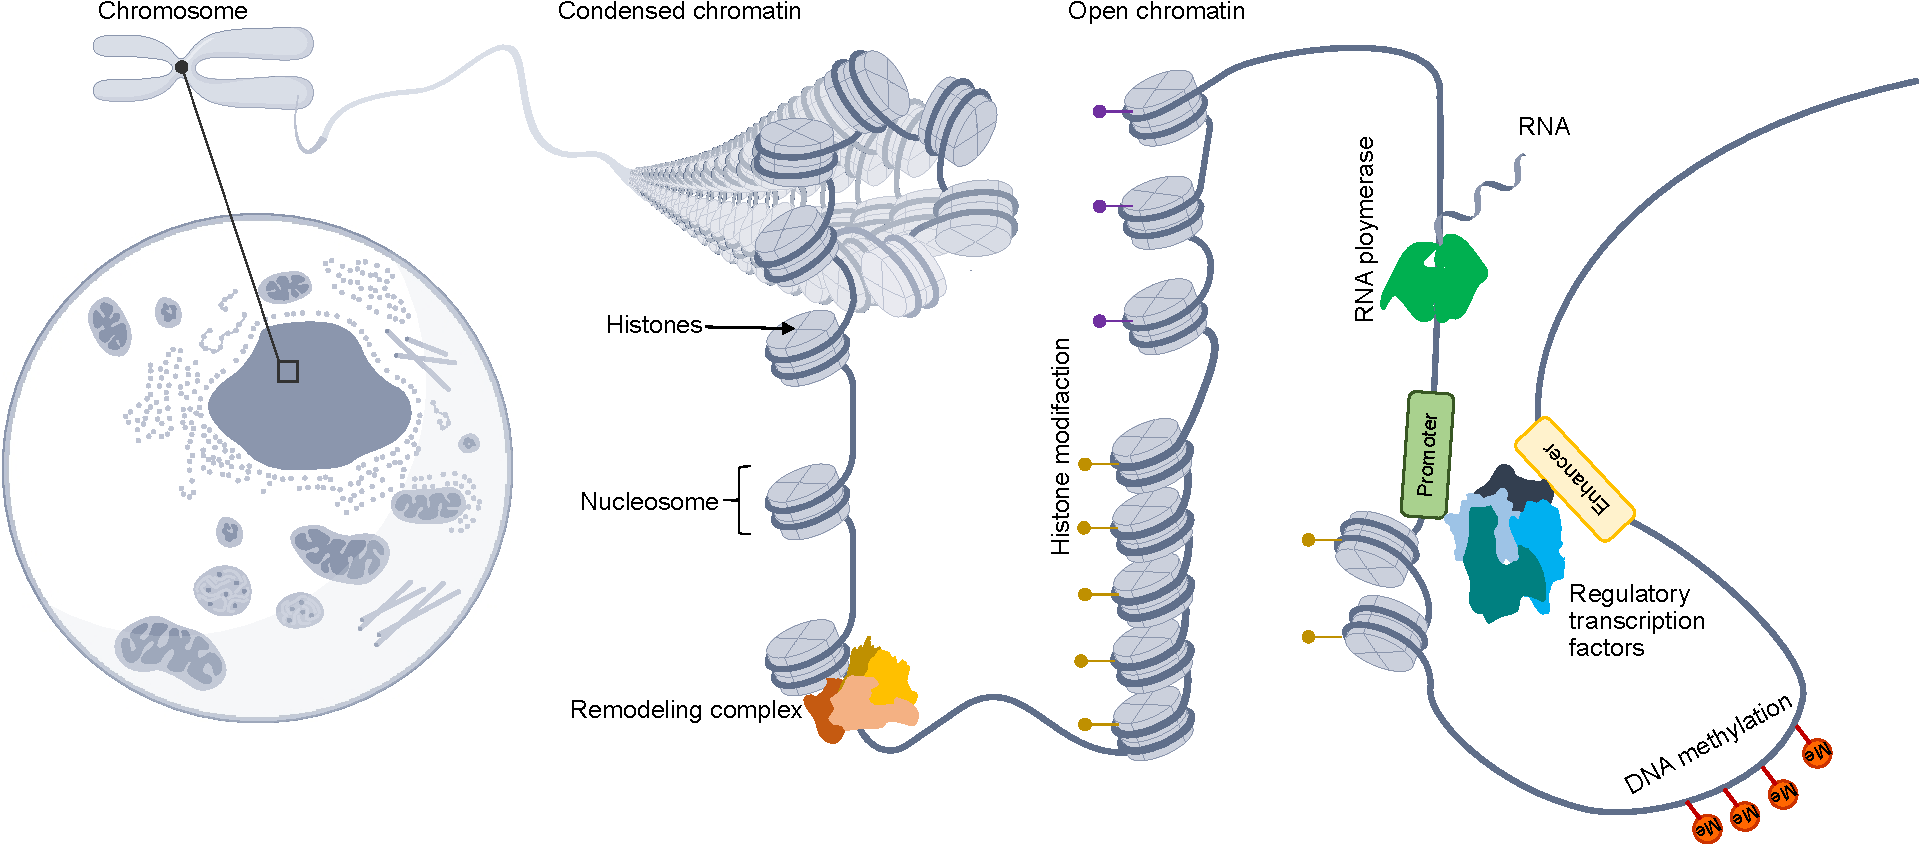
\includegraphics[width=0.95\textwidth]{chromatin_organization/fig}
	\vspace{0.1cm}
	\caption[DNA organization] {DNA is directed, controlled, and regulated by epistastic factors which surround and scaffold DNA in order to orchestrate the cellular mechanisms of life. The epigenome is the collection of DNA, RNA, proteins, and their chemical modifications that alter gene expression without changing the genetic code. Epigenetic machinery modifies the accessibility of regions in DNA by adding marks to the tails of histones, creating epigenetic patterns of chromatin modifications. The addition of an acetyl group to a histone tail changes the electrochemical charge of the histone, causing it to relax and release the DNA. This makes the DNA in that region more accessible to transcription machinery and allows that gene to be expressed. Placing a methyl group on histone tails can either increase or decrease the pattern of gene expression, depending on where the mark is placed. Additionally, placing a methyl group directly onto the DNA results in the permanent shutdown of that genetic region. \emph{Source:~\cite{heumos2023best}}~(modified to fit thesis format and/or clarify key points)}
	\label{fig:chromatin_organization}
\end{figure}


Chromatin is the complex of DNA and proteins found in the nucleus of a cell. Chromatin accessibility is a crucial molecular concept that describes the degree to which DNA is available or accessible for cellular processes, particularly gene expression. It can exist in two states: open and condensed. Open chromatin refers to the relaxed, accessible state where DNA is available for transcription and gene expression. In this state, the DNA is not tightly wound around histone proteins, allowing regulatory proteins and RNA polymerase to easily access specific DNA sequences, facilitating the transcription of genes into RNA. Open chromatin is associated with active gene expression and is influenced by various factors, including epigenetic modifications such as acetylation and methylation. Conversely, in a "closed" or condensed chromatin state, the DNA is covered with histone proteins, making it less accessible. This state inhibits the binding of transcriptional machinery, leading to reduced or suppressed gene expression. Closed chromatin is associated with inactive or silenced genes (\fref{fig:chromatin_organization}).




\section{Single cell sequencing technology}
\label{background:profiling_singlecell}
The invention of a series of rapidly evolving Next Generation Sequencing~(NGS) technologies revolutionarily facilitates the study of heterogeneous biological processes with high throughput, shorter time and lower cost~\citep{svensson2018exponential}. NGS enables researchers to perform profiling of epigenomes, transcriptomes and proteomes and the development of single-cell sequencing technology further facilitates the study of heterogeneity at single-cell resolution. In this section, we will briefly introduce single-cell sequencing technology, single-cell RNA sequencing, single-cell ATAC sequencing and single-cell protein sequencing.

To begin, let's establish clear definitions for genome, epigenome, transcriptome, and proteome. Genome is the complete set of DNA, which holds all the genetic information of an organism~\citep{hubbard2002genome}, epigenome is the complete set of reversible chemical changes to the DNA and histone proteins of an organism~\citep{bernstein2007epigenome}, transcriptome is the complete set of RNA molecules in a cell or a collection of cells~\citep{haoudi2006proteome}, proteome is the complete set of proteins expressed in a cell, tissue, or organism~\citep{wang2009transcriptome}. The term “-omics” refer to the exploration of corresponding omic data. Genomics specifically focuses on the investigation of an organism's genome. Likewise, epigenomics, transcriptomics, and proteomics encompass the study of epigenomes, transcriptomes, and proteomes, respectively.


\subsection{Transcriptomics profiling with scRNA-seq}
\label{background:sec1:scRNA}

Single-cell RNA sequencing~(scRNA-seq)~\citep{singlecellsequencing2014, singlecellsequencing2015} has emerged as a powerful tool that allows the study of gene expression at the individual cell level, providing insights into the heterogeneity and dynamics of cellular responses in various biological contexts. In contrast to traditional bulk RNA-seq, which averages gene expression across millions of cells, scRNA-seq enables the investigation of transcriptomic profiles within specific cell types, offering a more detailed understanding of cellular behaviors during development or in response to perturbations.

\begin{figure}[!ht]
	\centering
	\includegraphics[width=0.95\textwidth]{/scRNA_sequencing/fig}
	\vspace{0.1cm}
	\caption[Droplet-based simultaneous single-cell sequencing of transcriptome and epigenome.]{\textbf{Droplet-based simultaneous single-cell sequencing of transcriptome and epigenome.} \textbf{A)} The top left depicts Gel beads with a barcode fragment each. The bottom left shows a single nuclei suspension with single nuclei RNA and single nuclei ATAC-seq fragments. On the right, there's a Gel bead barcode that will attach to a single cell, forming a droplet. \textbf{B)} Four droplets are displayed, each containing a bead with a barcode fragment and a single cell. Barcodes uniquely identify individual cells. \textbf{C)} Droplets with single cells are isolated for sequencing, generating single cell RNA-seq and single ATAC-seq libraries. \textbf{D)} Sequencing outputs single cell ATAC-seq fragments, and alignment to reference DNA reveals fragment distributions with peaks at specific DNA positions. \textbf{E)} Sequencing also outputs single-cell RNA reads, identifying specific genes with each gene's molecular count tagged with a Unique Molecular Identifier (UMI). \textbf{F)} Counting the peaks in each single cell (cell barcode) constructs a peak-by-cell count matrix for scATAC-seq data. \textbf{G)} Counting the UMIs of each single cell (cell barcode) constructs a gene-by-cell count matrix for scRNA-seq data.}
	\label{fig:scRNA_scATAC_to_count_matrix}
\end{figure}

Single-cell RNA sequencing~(scRNA-seq) was introduced in 2009~\citep{tang2009mrna}. In general, scRNA-seq protocols can be classified into droplet-based and plate-based methods. Droplet-based methods use droplet microfluidics technology~\citep{dropletcompare2019, droplet2019practice} to capture cells in each droplet whereas plate-based methods employ passive cell separation into discrete wells on a plate. The droplet device is designed to generate aqueous droplets within mineral oil. Its arrangement strategically allows the simultaneous capture of cells and primed beads within a droplet, leading to the creation of an individual cDNA library for each cell. Each library is uniquely tagged with the barcode sequence present on the bead~(\fref{fig:scRNA_scATAC_to_count_matrix} A-C). Droplet-based capture technologies offer the advantage of capturing a significantly larger number of cells simultaneously, reaching up to tens of thousands. Additionally, these approaches exhibit reduced selectivity regarding cell size and generate fewer doublets. Thus, droplet-based techniques are currently the most commonly used cell capture technologies in single-cell RNA fields. We only focus on the droplet-based methods in this thesis.


\subsection{Chromatin accessibility profiling with scATAC-seq}
\label{background:sec1:scATAC}

Advancements in Next-Generation Sequencing~(NGS) technology have led to the development of various methods for comprehensive genome-wide profiling of chromatin accessibility through sequencing. ATAC-seq~(assay for transposase-accessible chromatin using sequencing)~\citep{buenrostro2013atacseq} use Tn5 transposase to insert sequencing adapters into accessible regions of the genome~(\fref{fig:ATAC-seq}). Due to the employment of a hyperactive Tn5 transposase, which tags and fragments DNA sequences in open chromatin regions simultaneously, ATAC-seq requires shorter sample preparation times and a lower number of cells for high-quality profiling of chromatin accessibility compared to other methods, ATAC-seq has gained prominence as the most extensively utilized~\citep{minnoye2021chromatin}.

\begin{figure}[!ht]
	\centering
	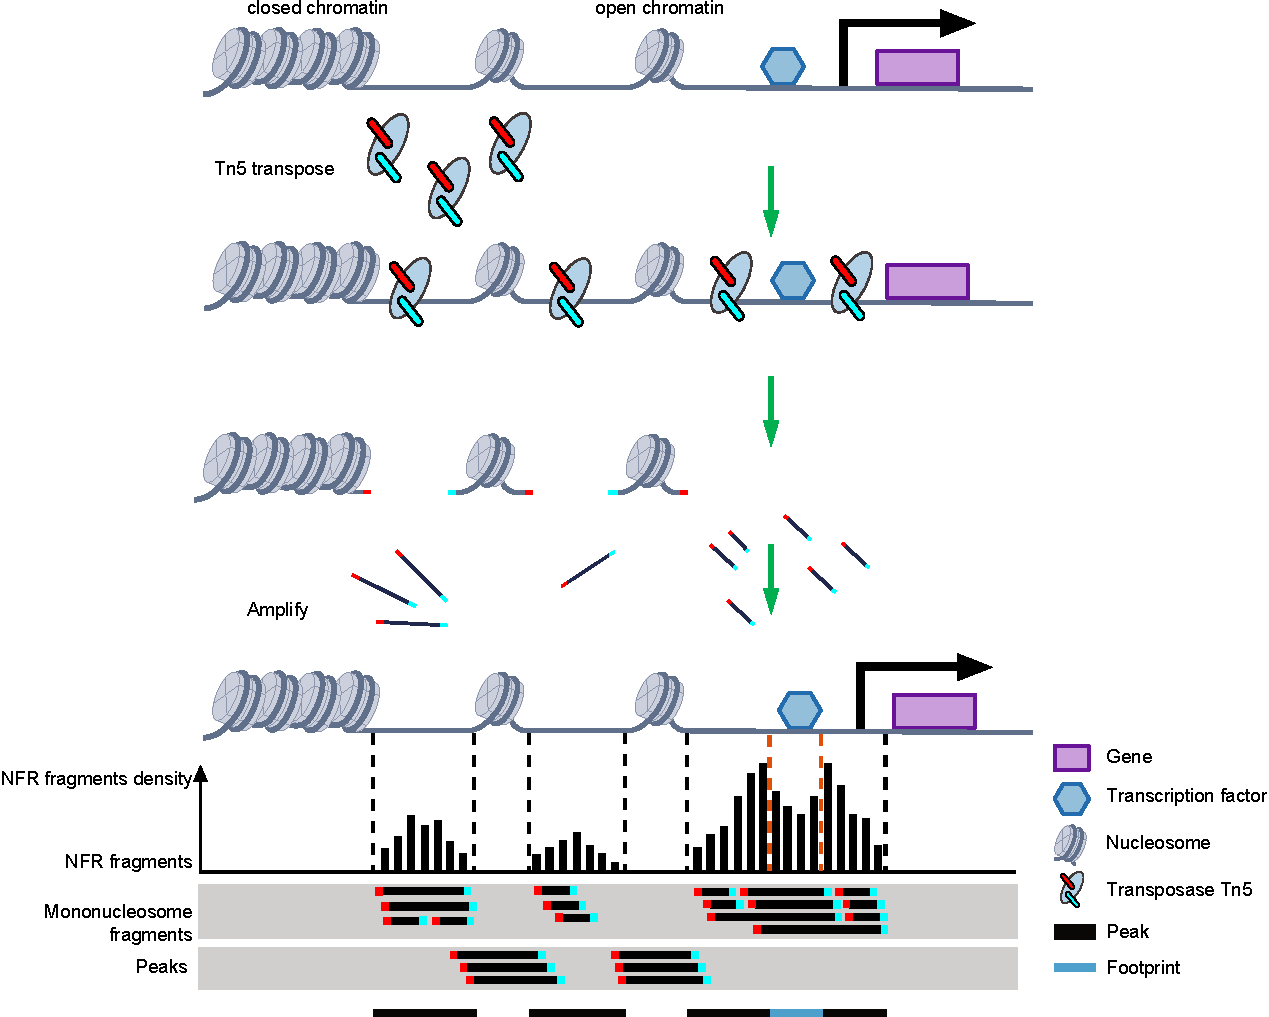
\includegraphics[width=0.85\textwidth]{scATAC-seq/fig}
	\vspace{0.1cm}
	\caption[ATAC sequenceing schematic flow.]{The ATAC-seq assay is employed for the identification of chromatin accessibility. Initially, the hyperactive Tn5 transposase selectively targets and modifies DNA regions characterized as "open" chromatin. Through a process known as tagmentation, the enzyme introduces sequencing adapters~(or priming sequences) into these open regions. Next, the resulting DNA fragments are amplified and input to high-throughput sequencing. \emph{Source:~\cite{yan2020reads}}~(modified to fit thesis format and/or clarify key points)}
	\label{fig:ATAC-seq}
\end{figure}

Protocols for single-cell ATAC-sequencing~(scATAC-seq) was introduced in 2015~\citep{Buenrostro2015,cusanovich2015multiplex}, enabling the unbiased identification of cell-type-specific regulatory elements within heterogeneous cell populations. Droplet-based scATAC-seq boasts a high throughput, capable of processing tens of thousands of cells per assay. Specifically, single nuclei are initially isolated from a single-cell suspension and subjected to bulk transposition with transposase Tn5. Following this, gel beads in emulsion~(GEM) are generated, with each gel bead being barcoded. Barcoded DNA fragments in droplets are finally used to create indexed libraries for high-throughput sequencing. Due to the advantages of high throughput and low costs for droplet-based single-cell ATAC-seq technology, the method is increasingly popular and has been commercialized by 10$\times$ Genomic~(Chromium Next Gem Single Cell ATAC-seq Library Kit)~\citep{satpathy2019massively}.



%\subsection{Protein profiling in single cell}
%\label{background:sec1:protein}
%%Protein analysis at the single-cell level has relied on the use of antibodies that bind specifically to target proteins. Flow cytometry uses fluorescently labeled antibodies to convert protein signals into fluorescence signals~\citep{@article{kim2022single}
%Secreted proteins play crucial roles in facilitating diverse biological processes, including cell–cell communication, differentiation, migration, and maintaining homeostasis at the population or tissue level. Methods for directly measuring specific protein-secreting cells in clinical settings include enzyme-linked immunospot~(ELISPOT) and its variants, such as fluorescence-based immunospot~(FluoroSpot)~\citep{perfetto2004seventeen, karlsson2003comparison}. Indirect assessment of protein secretion function can be conducted through intracellular staining using fluorescence-activated cell sorting~(FACS)~\citep{bonner1972fluorescence}. The detection of multiple cytokines in single cells has become possible through intracellular cytokine staining using multicolor flow cytometry~\citep{irish2004single,hale2009stage}. Mass cytometry is a deviation from traditional flow cytometry utilizing mass spectrometry for detection via rare earth metal probes, has demonstrated highly multiplexed measurement of surface and intracellular proteins~\citep{spitzer2016mass}.
%
%To comprehensively assess the expression patterns of individual proteins, researchers typically opt for mass spectrometry or flow cytometry rather than sequencing~\citep{kim2022single}. The application of mass spectrometry to single-cell proteomics poses technical challenges related to factors like required sample amounts and detection coverage. Efforts are underway to develop methods that enable the measurement of more protein molecules with lower sample input. In recent single-cell studies, CyToF, a mass cytometry-based method, has been employed to analyze dozens of surface and intracellular proteins using metal-labeled antibodies. Particularly beneficial for immune cells, profiling cell surface proteins aids in cell type classification. CyToF has been extensively utilized in studies, including those in general and cancer immunology, often in conjunction with scRNA-seq analysis~\citep{kashima2020single}.





\begin{figure}[!ht]
	\centering
	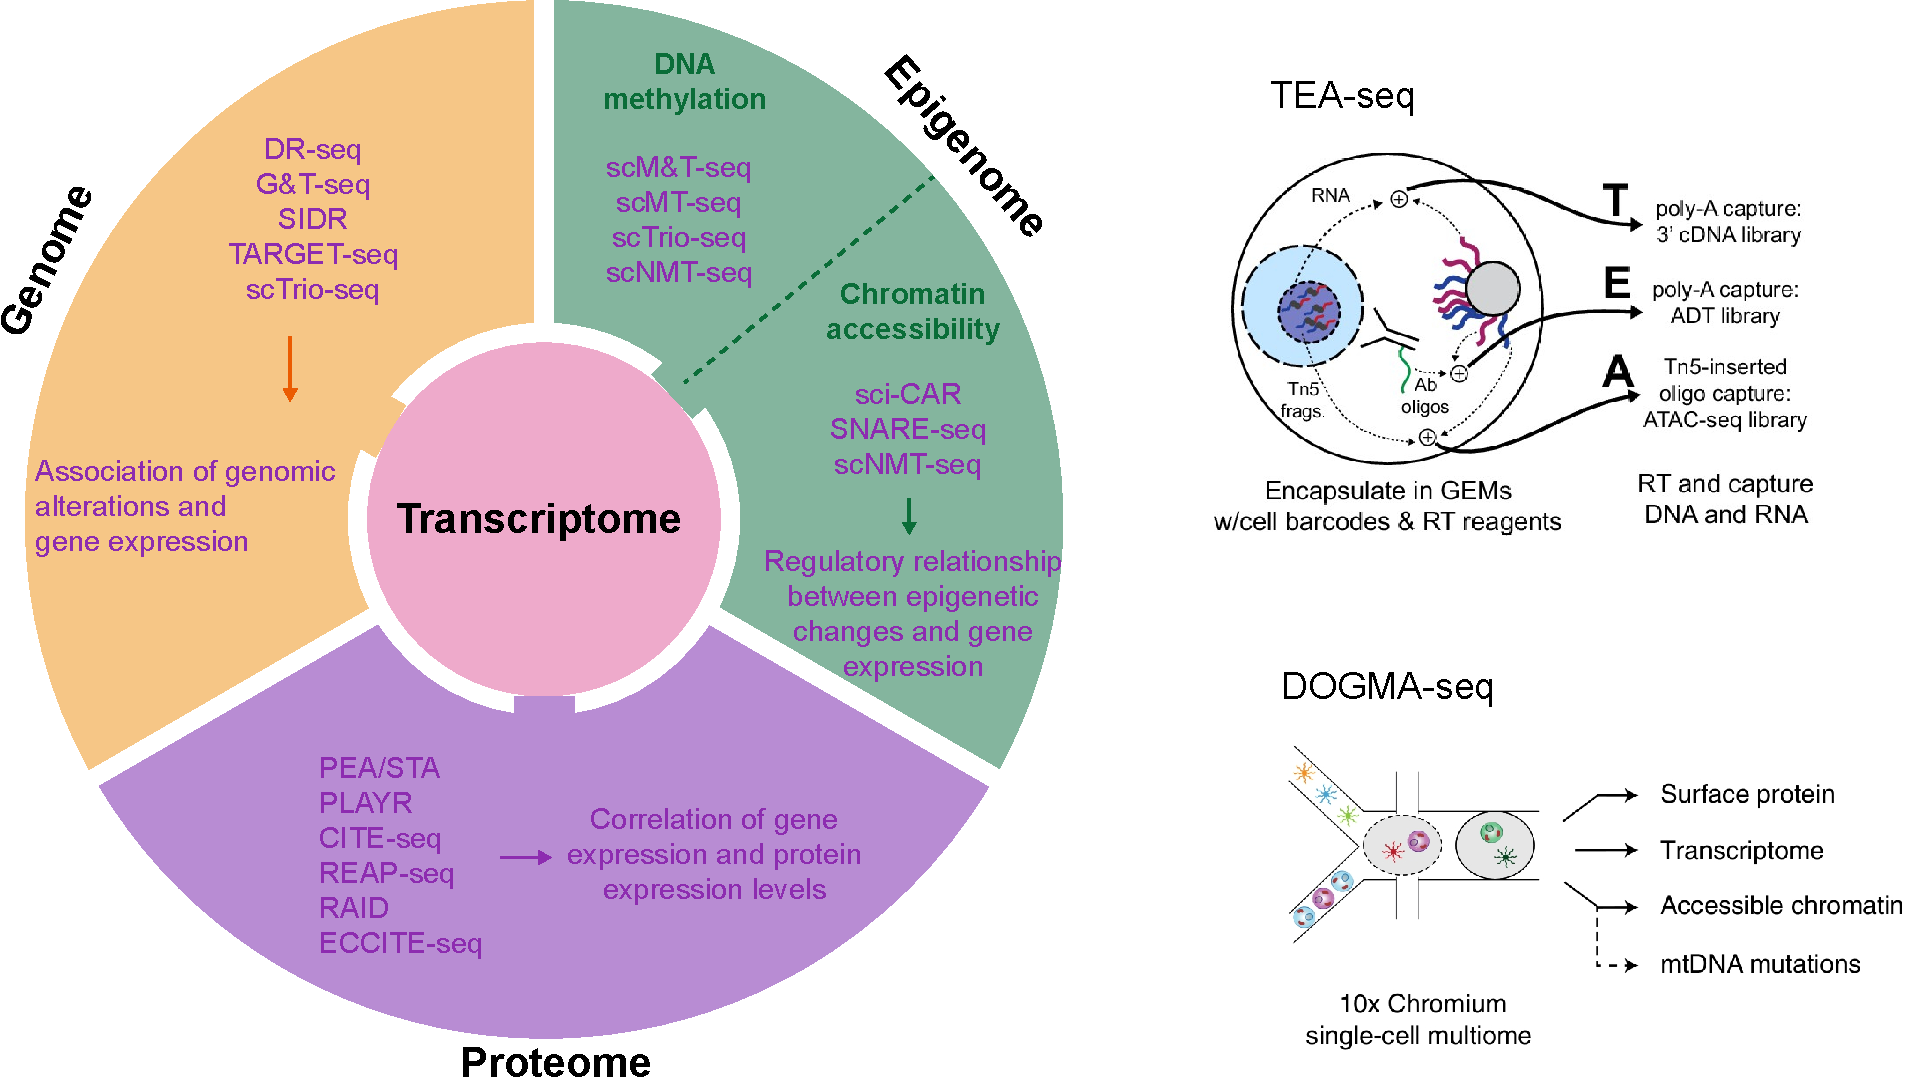
\includegraphics[width=0.50\textwidth]{multi-model-methods/fig}
	\vspace{0.1cm}
	\caption[multimodal methods protocols for Transcriptome, Genome, EpiGenome and Proteome]{multimodal methods protocols for Transcriptome, Genome, EpiGenome and Proteome. \emph{Source:~\cite{lee2020single}}~(modified to fit thesis format and/or clarify key points)}
	\label{fig:piechart-mulitmodal-methods}
\end{figure}



\subsection{Simultaneous multi-modal profiling of single cell}
\label{background:sec1:mulitmodal}
Single-cell multi-modal technologies typically analyze various types of molecules within a single cell, providing a more profound understanding of biology compared to studying individual molecular layers from separate cells. These advanced technologies unveil cellular heterogeneity across multiple molecular levels within a cell population, offering insights into the interconnectedness or independence of variation across different modalities. The datasets produced by these techniques hold the potential to facilitate a more comprehensive comprehension of the fundamental biological processes and mechanisms that contribute to cellular heterogeneity. Furthermore, they shed light on the associations between normal development, aging, disease etiology, and the intricate links between these phenomena. A variety of single cell multi-modal profiling methods have been proposed recently as shown in \tref{tab:multimodal-methods} and in \fref{fig:piechart-mulitmodal-methods}. We introduce these protocols by breaking down them into 3 groups:

\begin{itemize}
	\item \textbf{Transcriptome \& epigenome:}
	Several sequencing methods have been devised to simultaneously profile transcriptome and epigenome, E.g., single-cell combinatorial indexing chromatin accessibility and mRNA~(sci-CAR)~\citep{cao2018scicar}, single-nucleus chromatin accessibility and mRNA expression sequencing~(SNARE-seq)~\citep{chen2019SNARE}, and single-nucleus chromatin accessibility and RNA expression sequencing~(SHARE-seq)~\citep{ma2020shareseq}.


	\item \textbf{Transcriptome \& proteome:}
	Various methods have been developed, including proximity extension assay/specific RNA target amplification~(PEA/STA), proximity ligation assay for RNA~(PLAYR), cellular indexing of transcriptomes and epitopes by sequencing~(CITE-seq)~\citep{stoeckius2017citeseq}, and RNA expression and protein sequencing assay~(REAP-seq)~\citep{peterson2017reapseq}. Additionally, expanded CRISPR-compatible cellular indexing of transcriptomes and epitopes by sequencing~(ECCITE-seq)~\citep{mimitou2019ECCITE} is a modification and extension of CITE-seq, incorporating transcriptome, protein, clonotype, and CRISPR perturbation data at a single-cell resolution. To note, for the most common protocol CITE-seq, the sequencing data includes specific CITE-seq barcodes, also known as antibody-derived tags~(ADT), which identify the antibodies bound to the cells and provide information about the cell-surface proteins present~\citep{stoeckius2017citeseq}.

	\item \textbf{Transcriptome \& epigenome \& proteome:}
	Methods have been developed to profile more than two modalities, including TEA-seq~\citep{swanson2021simultaneous}, designed as a trimodal assay that simultaneously measures transcriptomics~(scRNA-seq), epitopes, and chromatin accessibility~(scATAC-seq) from thousands of single cells. Another method, DOGMA-seq~\citep{mimitou2021scalable}, can measure all features of TEA-seq and also detect mtDNA mutations simultaneously.

\end{itemize}

\begin{table}[!ht]
	\footnotesize
	\centering
	\begin{tabular}{lll}%{0.1\linewidth}}
		\toprule
		{\textbf{Modalities}} & {\textbf{Protocols}} & {\textbf{reference}} \\
		\midrule
		\multirow{5}{*}{\shortstack[l]{
\includegraphics[scale=.7]{multi-model-methods/Protein_RNA.pdf}}}
		  & PLAYR & {~\cite{frei2016playr}} \\
		  & CITE-seq & {~\cite{stoeckius2017citeseq}} \\
      & REAP-seq & {~\cite{peterson2017reapseq}}\\
      & RAID & {~\cite{Gerlach2019RAID}} \\
		  & ECCITE-seq & {~\cite{mimitou2019ECCITE}}\\
		\midrule
		\multirow{5}{*}{\shortstack[l]{
\includegraphics[scale=.7]{multi-model-methods/RNA_ATAC.pdf}}}
		  & sci-CAR & {~\cite{cao2018scicar}}\\
      & SNARE-seq & {~\cite{chen2019SNARE}} \\
      & scNMT-seq & {~\cite{clark2018scnmt}}\\
		  & scCAT-seq & {~\cite{liu2019scCAT}} \\
		  & SHARE-seq & {~\cite{ma2020shareseq}}\\
		\midrule
		\multirow{5}{*}{\shortstack[l]{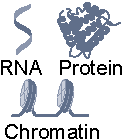
\includegraphics[scale=.7]{multi-model-methods/3.pdf}}}
		& TEA-seq & {~\cite{swanson2021simultaneous}}\\
		& DOGMA-seq &~\cite{mimitou2021scalable} \\
		\\
		\\
		\\
		\bottomrule
	\end{tabular}
	\vspace{0.1cm}
	\caption[Major multimodal methods]{major multimodal methods.}
	\label{tab:multimodal-methods}
\end{table}


\section{Computational analysis of single cell}
\label{background:computational_singlecell}
After designing the experiment and conducting the sequencing, the subsequent crucial step involves performing computational analysis to extract valuable insights from the single cell data. For scRNA-seq and scATAC-seq data, the initial step involves aligning the reads to the reference genome to identify gene expression or the location of the reads, respectively. Generally, after obtaining the feature count matrix~(features by cells), the analysis includes three steps: pre-processing for quality checks and normalization, dimensional reduction and clustering to identify heterogeneous population groups, and downstream analysis based on different feature properties. In this section, we will introduce these analyses by first discussing the alignments of scRNA-seq and scATAC-seq. Next, we describe the computational analysis of scRNA-seq, followed by the analysis of scATAC-seq data and that of the surface protein data.

\subsection{Alignment}
\label{background:sec2:alignment}
The first step in the computational analysis of ATAC-seq/RNA-seq is the alignment, in which, raw sequencing reads~(DNA for scATAC-seq, RNA for scRNA-seq) are aligned to the reference genome to ensure these reads are located in the most probable position of the reference genome. This is typically accomplished by constructing a large index database from a reference genome and/or the set of reads, identifying potential regions for pairwise alignment~\citep{alser2021alignment}. The most widely used aligners are Bowtie2~\citep{langmead2012bowtie2}, BWA~\citep{li2009BWA} and STAR~\citep{dobin2013star}. These tools are utilized in the Cell Ranger ATAC/RNA/ARC pipeline developed by 10$\times$ Genomics.

\subsection{Computational Analysis of Single Cell RNA-seq}
\label{background:sec2:scRNA}
We will outline the computational workflow for scRNA-seq data analysis, covering preprocessing~(quality control, normalization, feature selection), core analysis~(dimensionality reduction, batch correction, and clustering), and downstream analysis~(differential expression, cell annotation, trajectory analysis, and gene set enrichment).

\begin{figure}[!ht]
	\centering
	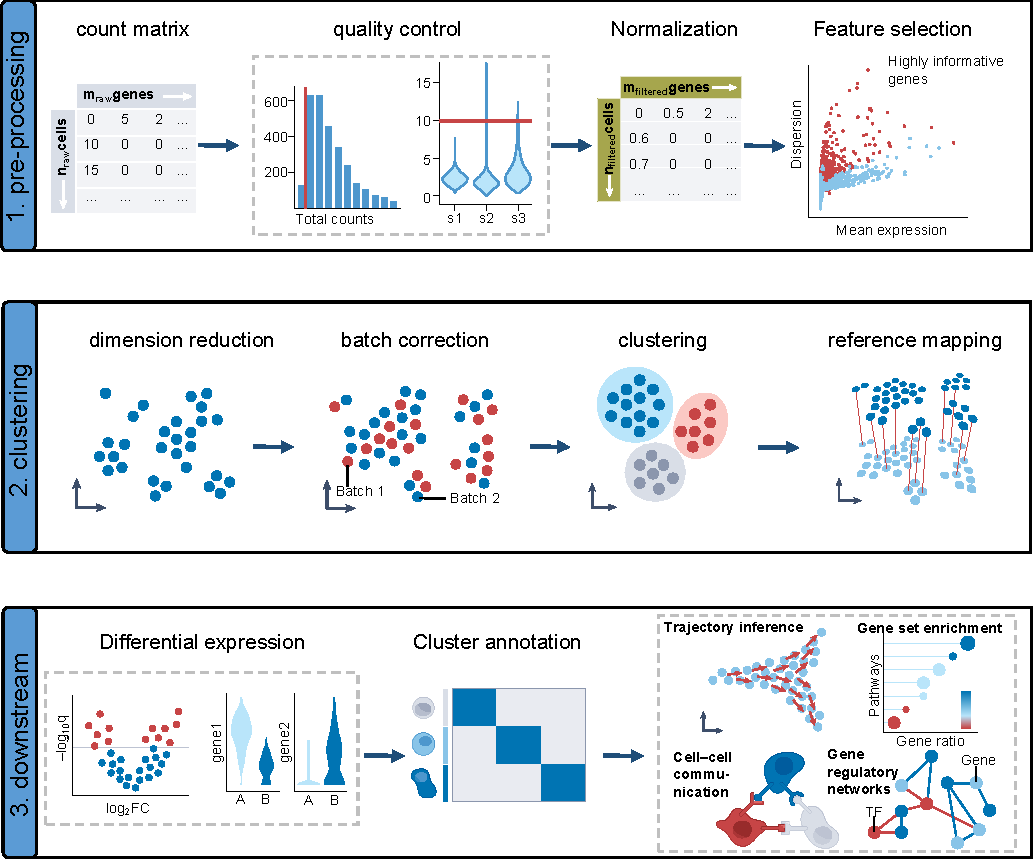
\includegraphics[width=0.85\textwidth]{workflow_scRNA/fig}
	\vspace{0.1cm}
	\caption[A common computational scRNA-seq analysis workflow]{
		\textbf{A common computational scRNA-seq analysis workflow}.
		\textbf{Step 1:} Preprocessing starts with cell by gene count matrix, including quality control, normalization and feature selection.
		\textbf{Step 2:} core analysis, including dimensionality reduction, batch correction and clustering and reference mapping.
		\textbf{Step 3:} Downstream analysis, including differential expression, cell annotation, trajectory analysis and geneset enrichment.
	workflow scRNA. \emph{Source:~\cite{heumos2023best}}~(modified to fit thesis format and/or clarify key points)}
	\label{fig:workflow_scRNA}
\end{figure}

\subsubsection{Pre-processing}
We start from a count matrix where the mRNA sequence reads obtained are aligned to genes and cells of origin through an alignment pipeline e.g 10$\times$ cellranger pipeline~\citep{zheng2017massively}. The pipeline utilizes either cellular barcodes or unique molecular identifiers~(UMIs) in conjunction with a reference genome. We eventually obtain a count matrix representing cells by genes.
\begin{description}
	\item[Quality Control]
	We focus on droplet-based scRNA data quality control. \fref{fig:QCcells}A shows an intact droplet, where a droplet includes a cell and barcode bead to mark the cell ID. The objective of quality control is to filter low-quality cells~(\fref{fig:QCcells}B-E) and correct the noise. Cells characterized by a low number of detected genes, a shallow count depth, and a high proportion of mitochondrial counts are commonly referred to as low-quality cells. This designation is often indicative of cells in a state of decline, potentially exhibiting compromised membranes associated with cell damage or death. Low-quality cells are detected and filtered by manually setting thresholds, as suggested in a guide~\citep{luecken2019current}. Doublets or multiplets occur when more than one cell is present in a droplet~(\fref{fig:QCcells}D). The simplest method to address this issue is to filter out cells with an excessively high total count of gene molecules~(UMI). More sysmatic approach involves creating synthetic doublets by combining two cells and examining the neighborhoods of cells to detect potential doublets~\citep{mcginnis2019doubletfinder}. Ambient RNA removal typically involves using the expression profile of empty droplets to eliminate background noise from cells~\citep{janssen2023benchambient}.


	\item[Normalization]
	Cells may exhibit varying numbers of gene counts due to disparities in cell size or random variations during sequencing. Count normalization is employed to ensure comparability in cellular profiles. A common normalization method involves dividing the raw UMI count by the total detected RNAs in each cell, multiplying the result by a scaling factor~(typically set at 10,000), adding a pseudo-count~(usually 1), and subsequently applying a log transformation to the outcome. This size-factor normalization effectively mitigates technical variations arising from sequencing depth, while the log transformation serves to alleviate the impact of expression outliers. This approach is particularly valuable in preventing high-abundance genes from disproportionately influencing downstream analyses due to their elevated technical variability. Log-normalization is the default method in the most popular single cell analysis toolkit Seurat~\citep{stuart2019seurat3} written in R and Scanpy~\citep{wolf2018scanpy} implemented in python.

	\item[Feature Selection]
	Single-cell RNA-seq datasets typically contain more than 20,000 genes. Numerous genes lack informativeness and predominantly consist of zero counts. Thus, feature selection is necessary to select the most informative features~(usually 3,000$\sim$5,000 genes) and reduce the computing resources and data dimensions, as well as alleviate issues such as model overfitting in downstream analysis~\citep{yang2021feature}. The objective is to exclude uninformative genes that may not reflect meaningful biological variation across samples. The commonly used method is implemented in Seurat, where genes are categorized based on their average expression. The gene with the highest ratio of variance to mean within each group is selected as the Highly Variable Gene~(HVG) for that specific bin~\citep{stuart2019seurat3}.
\end{description}

\begin{figure}[!ht]
	\centering
	\includegraphics[width=0.65\textwidth]{QC_cells/fig}
	\vspace{0.1cm}
	\caption[Droplets-based sequencing of cells in low quality.]{\textbf{Droplets-based sequencing of cells in low quality.} Droplet-based protocols for single-cell analysis require rigorous quality checks to ensure accurate downstream analysis. \textbf{A)} An intact droplet should ideally contain a single cell and a corresponding barcode for cell identification. \textbf{B)} Contamination may occur through the introduction of ambient RNA, leading to the inclusion of extraneous RNA reads not originating from the targeted cell. \textbf{C)} Droplets capturing dying cells typically exhibit lower levels of detected RNA reads, indicating compromised cell integrity. \textbf{D)} Occasionally, a droplet may capture more than one cell, posing challenges for subsequent analysis. \textbf{E)} Empty droplets, which capture no cells with extremely few gene expressions, are easily identified and can be excluded from analysis. These considerations emphasize the importance of thorough quality control measures in droplet-based single-cell protocols to ensure the reliability and accuracy of the generated data. \emph{Source:~\cite{heumos2023best}}~(modified to fit thesis format and/or clarify key points)}
	\label{fig:QCcells}
\end{figure}
\subsubsection{Dimensional reduction and clustering}
\label{background:sec2:dr_n_clustering}
\begin{description}
	\item[Dimensional Reduction]
	Dimensional reduction serves a dual purpose: preserving distances between cells with lower dimensions and facilitating data visualization. In the context of single-cell RNA sequencing~(scRNA-seq), Principal Component Analysis~(PCA)~\citep{hotelling1933pca} is often employed to reduce dimensionality, transforming high-dimensional data by maximizing the residual variance captured in each potential dimension. Subsequently, Uniform Manifold Approximation and Projection~(UMAP) or t-distributed Stochastic Neighbor Embedding~(t-SNE) are commonly utilized for data visualization with 2 dimensions preserved. However, both methods do not accurately represent the real distances between cells and should not be used for downstream analysis~\citep{mcinnes2018umap, van2008tsne}.

	\item[Batch Correction]
	Batch effects are a common confounding factor in single-cell RNA-seq experiments. Namely, they are systematic differences in measurements between batches~(e.g., technical replicates, different days of lab work, different individuals, etc.) that are not due to the biological signal of interest. Batch effects can be caused by a variety of factors, including differences in reagents, equipment, and personnel. Numerous methods have been proposed to address batch effects. Seurat employs canonical correlation analysis~(CCA) to identify anchors between batches, utilizing these anchors for subsequent correction~\citep{stuart2019seurat3}. Scanpy uses batch-balanced k-nearest neighbors~(BBKNN) to identify mutual nearest neighbors across batches, facilitating batch effect correction~\citep{polanski2020bbknn}. Harmony addresses batch effects by iteratively clustering similar cells from different batches at each iteration, maximizing batch diversity within clusters, and calculating correction factors for subsequent application~\citep{korsunsky2019harmony}. Comparative evaluations of batch correction methods indicate Harmony's superior performance~\citep{tran2020benchmark}.

	\item[Clustering]
	With the batch-corrected data, we can proceed to cluster cells into groups with similar expression profiles, elucidating the heterogeneity in the dataset. Various methods have been proposed for clustering, with graph-based clustering being particularly popular. For instance, Seurat utilizes the Louvain algorithm as its default clustering method~\citep{stuart2019seurat3}, while Scanpy defaults to the Leiden algorithm~\citep{traag2019louvain}. An independent benchmarking study of clustering methods revealed that SC3~\citep{kiselev2017sc3} and Seurat demonstrated the overall best performance and were the only ones to accurately recover cell types in droplet-based datasets~\citep{duo2018benchclustering}.

\end{description}

\subsubsection{Downstream analysis}
\begin{description}
	\item[Differential Gene Expression]
	Differential gene expression aims to identify genes that exhibit significant expression differences between clusters or conditions. These genes contribute valuable information for annotating cell types within clusters and interpreting biological distinctions influenced by specific conditions. The Wilcoxon rank-sum test stands out as the most widely used method for identifying differentially expressed genes, with the Student's t-test occasionally employed for this purpose. Other models, such as MAST, utilize the hurdle model to identify differentially expressed genes~\citep{finak2015mast}. Popular single-cell RNA analysis toolkits like Seurat and Scanpy have incorporated various statistical methods, including the Wilcoxon rank-sum test, t-test, and linear models like logistic regression, to identify genes exhibiting differential expression.

	\item[Cluster Annotation]
	With the clusters and significant gene markers of each cluster, identifying the cell types of each cluster is essential, requiring domain knowledge and an understanding of the biological context. The most prevalent approach to annotating cell types involves using marker genes—genes that exhibit high expression levels in specific cell types. Biologists can curate marker genes by identifying genes significantly highly expressed through differential gene expression analysis, aiding in the annotation of heterogeneous cell groups. Cluster annotation stands as a pivotal task in single-cell analysis, playing a crucial role in identifying cell types and interpreting the biological meaning of distinct cell groups.

	\item[Trajectory Inference]
	Trajectory inference, also known as pseudotemporal ordering, is a computational technique employed in single-cell transcriptomics to elucidate the pattern of a dynamic process undergone by cells. Trajectory inference arranges cells based on their progression through the identified process. Note that various subtasks of trajectory inference have been addressed by researchers, with dimension reduction being a critical aspect. Exclusive dimension reduction is essential due to the potential distortion of the global structure by nonlinear visualization methods like t-SNE and UMAP. Approaches such as multidimensional scaling~(MDS)~\citep{torgerson1952multidimensional} aim to reduce dimensions while preserving distance information in a 2 dimensional space, and diffusion maps~\citep{coifman2006diffusion} utilize Gaussian affinities to capture both local and global structural details. PHATE, developed by~\cite{moon2017phate}, leverages both local and global structure. Palantir employs a forced-directed layout to Gaussian affinities within a graph. Pseudotime simulation is another aspect focused on capturing the temporal order of differentiating cells. Diffusion pseudotime~(DPT), introduced by~\citep{haghverdi2016dpt}, measures transitions between cells using diffusion-like random walks and has been integrated into the popular Python single-cell toolkit Scanpy~\citep{wolf2018scanpy}. Additionally, methods like slingshot~\citep{street2018slingshot} and STREAM~\citep{chen2019stream} are explored in more detail in \sref{background:sec2:TI}.

	\item[Gene set Enrichment]
	Gene set enrichment analysis facilitates the summarization of numerous molecular insights into interpretable terms, such as pathways, which are defined as sets of genes known to be involved based on previous studies. Commonly used databases for this purpose include MSigDB~\citep{liberzon2011msigdb}, Gene Ontology~\citep{gene2004go}, KEGG~\citep{kanehisa2007kegg}, and Reactome~\citep{fabregat2018reactome}.
\end{description}

\subsection{Computational Analysis of Single Cell ATAC-seq}
\label{background:sec2:scATAC}
In many cases, single-cell ATAC-seq data analysis is similar to single-cell RNA-seq, with some distinctions due to feature differences present in scATAC. Firstly, the features, represented as a cell-by-peak matrix, are typically more sparse and have a larger feature space~(\fref{fig:modalities_differences}). This necessitates different strategies for feature normalization, feature selection, and dimensional reduction. Secondly, scATAC-seq features are not gene expressions, posing a challenge for cell annotation and data interpretation. Lastly, due to these feature differences, the biological insights obtained from scATAC-seq differ from those of scRNA-seq, giving rise to different downstream analyses like linkage analysis or motif discovery.

We will describe the computational workflow for scATAC-seq data analysis, including, feature matrix construction, preprocessing~(feature definition, quality control, feature selection), core analysis~(dimensionality reduction, batch correction and clustering), and downstream analysis~(differential accessibility, trajectory inference etc. ).

\begin{figure}[!ht]
	\centering
	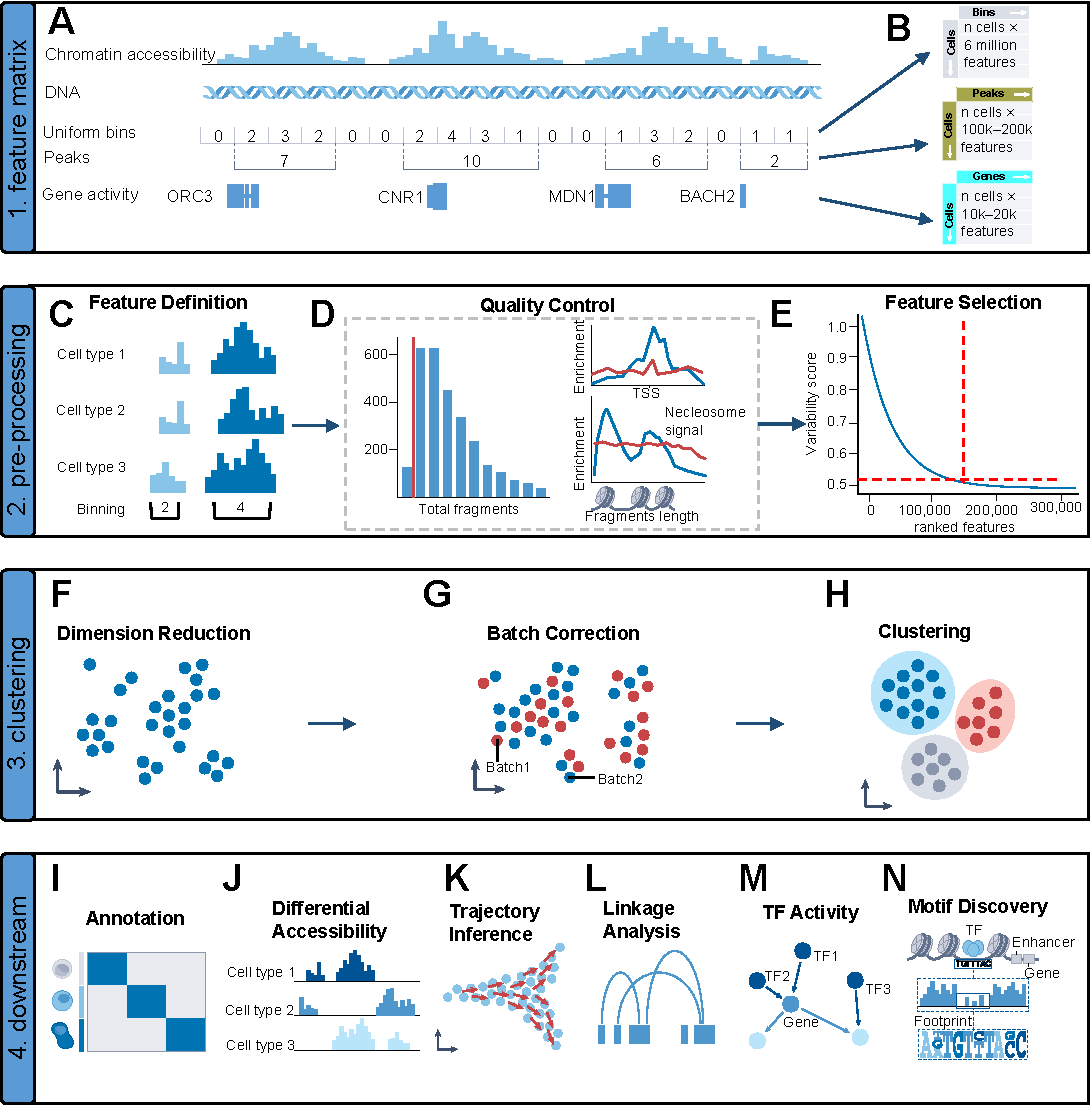
\includegraphics[width=0.85\textwidth]{workflow_scATAC/fig}
	\vspace{0.1cm}
	\caption[A common computational scATAC-seq analysis workflow]{
	\textbf{A common computational scATAC-seq analysis workflow:}
	\textbf{Step 1:} Feature matrix construction using peaks, bins or gene accessibility.
	\textbf{Step 2:} Preprocessing including feature selection, quality control, and feature selection.
	\textbf{Step 3:} Core analysis including dimensional reduction, batch correction, clustering, label transferring, and cell type annotation.
	\textbf{Step 4:} Downstream analysis including differential accessibility, trajectory inference, linkage analysis, TF activity and Motif discovery.

	\emph{Source:~\cite{heumos2023best}}~(modified to fit thesis format and/or clarify key points)}
	\label{fig:workflow_scATAC}
\end{figure}

\subsubsection{Feature matrix construction}
\label{background:sec2:scATAC:matrixconstruction}
In contrast to scRNA-seq data, which relies on clearly defined gene features, scATAC-seq data lacks a standardized feature set owing to the genome-wide nature of the data. Here we present three ways of feature matrix construction~(\fref{fig:workflow_scATAC}A). Most workflows typically utilize a cell-by-peak or cell-by-bin matrix as a foundation for analysis~\citep{heumos2023best}. However, it's important to note that the feature number in single-cell ATAC-seq is significantly larger compared to scRNA gene expression, usually reaching around 100,000 for this type of feature~(\fref{fig:modalities_differences}A). Another feature matrix gene activity score matrix can also be created to approximate gene expression, facilitating the interpretation of the data. We will outline how to construct these three feature matrices:
\begin{description}
	\item[Peak Matrix]
	Cell-by-peak is the most prevalent features for scATAC-seq data analysis. Peaks denote variable regions of open chromatin characterized by an enrichment of Tn5 transposition events compared to background noise. Note that the identification of peaks requires an adequate number of cells. Therefore, challenges may arise when dealing with rare cell types. To improve the sensitivity of peak detection, it is beneficial to call peaks within clusters. This approach mitigates the risk of overlooking peaks in rare cell types that might otherwise be obscured by the noise from more prevalent cell types. Currently, the most frequently employed peak caller for ATAC-seq is MACS2~\citep{zhang2008macs2} which was originally developed for ChIP-seq data, MACS2 utilizes a dynamic Poisson distribution to account for local background biases in the genome, enabling effective peak detection. Another peak caller HMMRATAC~\citep{tarbell2019hmmratac} which is a Hidden Markov Model-based method for ATAC-seq, employs a ``decomposition and integration'' approach to identify open chromatin regions by learning relationships between layers of coverage signals in a single ATAC-seq dataset. To note, 10$\times$ cellranger pipeline delivers a default cell-by-peak matrix output~\citep{satpathy2019massively}. R tool Signac~\citep{signac} and Python tool Episcanpy~\citep{Danese2021episcanpy} use cell-by-peaks features to do the analysis.

	\item[Bin Matrix]
	To generate a cell-by-bin count matrix, the genome is segmented into uniform-sized bins~(typically 500 bps). Single-cell ATAC-seq profiles are then represented as a cell-by-bin matrix, where each element indicates the number of sequencing fragments overlapping with a specific bin in a particular cell. This bin matrix is employed in scATAC-seq toolkits such as snapATAC~\citep{fang2021snapatac} and ArchR~\citep{Granja2021}.

	\item[Gene Score Matrix]
	Gene activity score is a prediction of how highly expressed a gene will be based on the accessibility of regulatory elements in the vicinity of the gene. Signac~\citep{signac} extracts gene coordinates and extends them to include the 2 kb upstream region~(as promoter accessibility is often correlated with gene expression) and then counts the number of fragments for each cell that map to each of these regions. Whereas ArchR~\citep{granja2019single} creates a tile matrix using a user-defined tile size~(default is 500 bp), overlaps these tiles with the user-defined gene window~(default is 100 kb on either side of the gene), and then calculates the distance from each tile~(start or end) to the gene body, with optional extensions upstream or downstream, or to the gene start.
\end{description}

\subsubsection{Pre-processing}
\begin{description}
	\item[Quality control]
	Similar to single-cell RNA sequencing, the number of fragments per cell serves as a crucial metric for filtering low-quality cells in single-cell ATAC-seq. A low number of fragment reads suggests low-quality cells, while an excessively high number might indicate potential doublets. Additionally, the enrichment of transcription start sites~(TSS)~\citep{Granja2021} is commonly employed as a filtering criterion. Other metrics, such as the fraction of reads in peaks~(FRiP), the ratio of reads in promoter regions and the ratio of reads in blacklist sites, are also utilized for quality checks in scATAC-seq data. Empirically, for human and mouse data, common quality thresholds include requiring the number of unique nuclear fragments to be greater than 1000, ensuring the FRiP is greater than 0.3, and targeting TSS enrichment scores greater than 5 or 6. The threshold should be determined based on the characteristics of samples in practice. Doublets detection is also necessary for scATAC-seq data. ArchR~\citep{Granja2021} also implemented a doublets detection function. It generates synthetic doublets in silico by blending the reads from thousands of combinations of individual cells and finding their nearest neighbors to identify doublets whose signals closely resemble those of the synthetic doublets.

	\item[Normalization]
	For scATAC data, we typically employ the term-frequency inverse-document-frequency~(TF-IDF) method for normalization. This method transforms a cell-to-feature
	matrix by assigning greater weight to rarer peaks within the cell population. The resulting transformed data matrix tends to emphasize peaks that demonstrate higher variability, enhancing their informativeness for distinguishing between different cell types. Widely-used scATAC-seq toolkits such as Signac~\citep{signac} and ArchR~\citep{granja2019single} both utilize TF-IDF for normalizing the count matrix.


	\item[Feature Selection]
	Given the typically larger number of peaks compared to genes in scATAC-seq data, effective feature selection is crucial. A common approach involves selecting peaks with high variance across cells, with methods like Signac~\citep{signac} utilizing the variance of the TF-IDF transformed matrix for peak selection.
\end{description}
\subsubsection{Dimensional reduction and Clustering}
\begin{description}
	\item[Dimensional Reduction]
	Unlike the scRNA data, scATAC usually uses different strategies to reduce the dimensions. The most commonly used Latent semantic indexing~(LSI) was first introduced for the analysis of scATAC-seq data by~\cite{cusanovich2015multiplex}. It combines the steps of TF-IDF followed by Singular value decomposition~(SVD). Signac~\citep{signac} use LSI as the default dimension reduction method, whereas ArchR implemented Iterative Latent Semantic Indexing~(iterativeLSI)~\citep{satpathy2019massively, granja2019single} which initiates by performing an initial Latent Semantic Indexing~(LSI) transformation on the most accessible bins and identified lower-resolution clusters that remain unaffected by batch confounding. To note, the first component of Latent Semantic Indexing~(LSI) in scATAC-seq data often captures sequencing depth. It is recommended to assess the correlation between each component and sequencing depth to exclude noise introduced for downstream analysis, as suggested by Signac~\citep{signac}. For visualization purposes, UMAP and t-SNE can be used, similar to single-cell transcriptomics.

	\item[Batch Correction \& Clustering]
	Similar to scRNA, see \sref{background:sec2:dr_n_clustering}.


\end{description}
\subsubsection{Downstream analysis}
\label{background:sec2:atac_downstream}
\begin{description}

	\item[Annotation]
	Without gene expression features, it's a challenge to annotate the cell types of each cluster. One way is to transfer labels from previous studies to scATAC data. Typically, this is achieved by integrating scATAC with existing scRNA data. For instance, methods provided by Seurat~\citep{stuart2019seurat3} find shared nearest neighbors from different studies to transfer labels~\citep{stuart2019seurat3}. Another approach involves using multimodal data as a molecular bridge, facilitating the mapping of scATAC onto scRNA-seq references~\citep{hao2023dictionary}. Apart from label transferring, we can also use gene activity score~(\sref{background:sec2:scATAC:matrixconstruction}) differentiation to identify cell types for each cluster. The Transcription Factor~(TF) motif enrichment score can be also used to assit the identification of the cell types.

	\item[Differential Accessibility]
	To gain insights into cluster/cell type-specific biology, one can perform differential accessibility analysis, akin to scRNA differential gene expression. Various statistical methods have been employed for this task, including the aforementioned Wilcoxon test from scRNA, which is also applicable here. Additionally, binomial tests~\citep{cusanovich2018single}, and logistic regression models~\citep{hao2021seurat4} are commonly used in scATAC-seq tools. Typically, methods for differential accessibility take into account the removal of technical biases, such as unique nuclear fragments and TSS enrichment. ArchR~\citep{Granja2021} selects a set of background cells that match the known biases for each cell group and performs comparisons between each cell group and its background cells. Signac~\citep{hao2021seurat4} employs logistic regression for differential accessibility analysis and treats the total number of fragments as a latent variable to mitigate the effects of technical biases.

	\item[Trajectory Inference]
	Trajectory analysis has been discussed in \sref{background:sec2:scRNA}.


	\item[Linkage Analysis]
	Accessibility profiles along the linear genome in individual cells have been shown to correlate with higher-order chromosome folding~\citep{Buenrostro2015}. Consequently, scATAC-seq data enables the extraction of promoter–enhancer interactions and gene regulatory networks through linkage analysis. Two main types of linkage analysis are peak-to-peak co-accessible analysis and peak-to-gene linkage analysis. Cicero~\citep{pliner2018cicero} is an algorithm designed for establishing genome-wide connections between distal enhancers and promoters based on co-accessibility patterns in scATAC-seq data. Peak-to-peak co-accessibility analysis seeks correlations of accessibility between two peaks across cells, but it doesn't necessarily indicate a direct regulatory relationship due to frequent co-accessibility of cell type-specific peaks. To overcome this, peak-to-gene linkage analysis integrates scRNA-seq data, calculating correlations between peak accessibility and gene expression~\citep{Granja2021}. This method, compared to peak-to-peak co-accessibility analysis, more accurately reflects gene regulatory interactions~\citep{shi2022scatacoverview}.

	\item[Motif Discovery]
	The binding of transcription factors to cis-regulatory DNA sequences controls gene expression programs and the dynamics during development or in disease. To compute transcription factor~(TF) binding site enrichment scores at the single-cell level, chromVAR~\citep{schep2017chromvar} assesses the accessibility deviation across all motif-containing peaks per cell while correcting for the Tn5 transposase's insertion bias. This bias arises from the sequence binding preferences of the transposase.

\end{description}

%%might ignore the surface protein part
\subsection{Computational Analysis of Single Cell Surface Protein}
\label{background:sec2:protein}
The feature size of surface protein is much smaller~(around 100) compared to other modality types~(\fref{fig:modalities_differences}A). It is often profiled together with scRNA-seq e.g., CITE-seq~\citep{citeseq2017} simulatenously profiles scRNA and suface protein.

Surface protein profilling outputs antibody-derived tags~(ADT) count matrix, which exhibits higher density compared to scRNA-seq and scATAC-seq data. For quality check, it is advisable to remove libraries with zero counts for the entire or a majority of the antibody panel~\citep{amezquita2020adtqc}. For protocols that simultaneously measure RNA and ADTs, such as CITE-seq~\citep{citeseq2017}, quality control for RNA and ADTs should be conducted separately. Since antibody efficacy can vary, batch correction of ADT data across multiple studies should also be performed~\citep{zheng2022adtqc}. To address biases in cell composition, normalization techniques such as centered log-ratio~(CLR) transformation is recommended~\citep{stoeckius2017citeseq}. The downstream analysis of ADT data follows a similar pipeline to unimodal RNA analysis, wherein annotated clusters can be tested for differential abundance.


%\section{Related works}
%\label{background:related_works}
\section{Computational Analysis of Single Cell Multimodal Omics}
\label{background:multimodal}
Computationally, multimodal single-cell omics profiling has paved the way for developing models that can capture interactions and associations among multiple modalities at single-cell resolution. In this section, We begin by presenting the common workflow of single-cell multimodal analysis. Following that, we delve into two crucial computational tasks: integration and trajectory inference for single-cell multimodal data. We will outline the challenges, current approaches, and our objectives to address these issues.

\subsection{Common Workflow of Single Cell Multimodal Omics}
\label{background:multimodal:workflow}
We will outline the computational workflow for the analysis of single-cell multimodal data. As depicted in \fref{fig:workflow_multimodal}, two crucial challenges, namely data integration and trajectory inference, need to be addressed during single-cell multimodal analysis.

\begin{figure}[!ht]
	\centering
	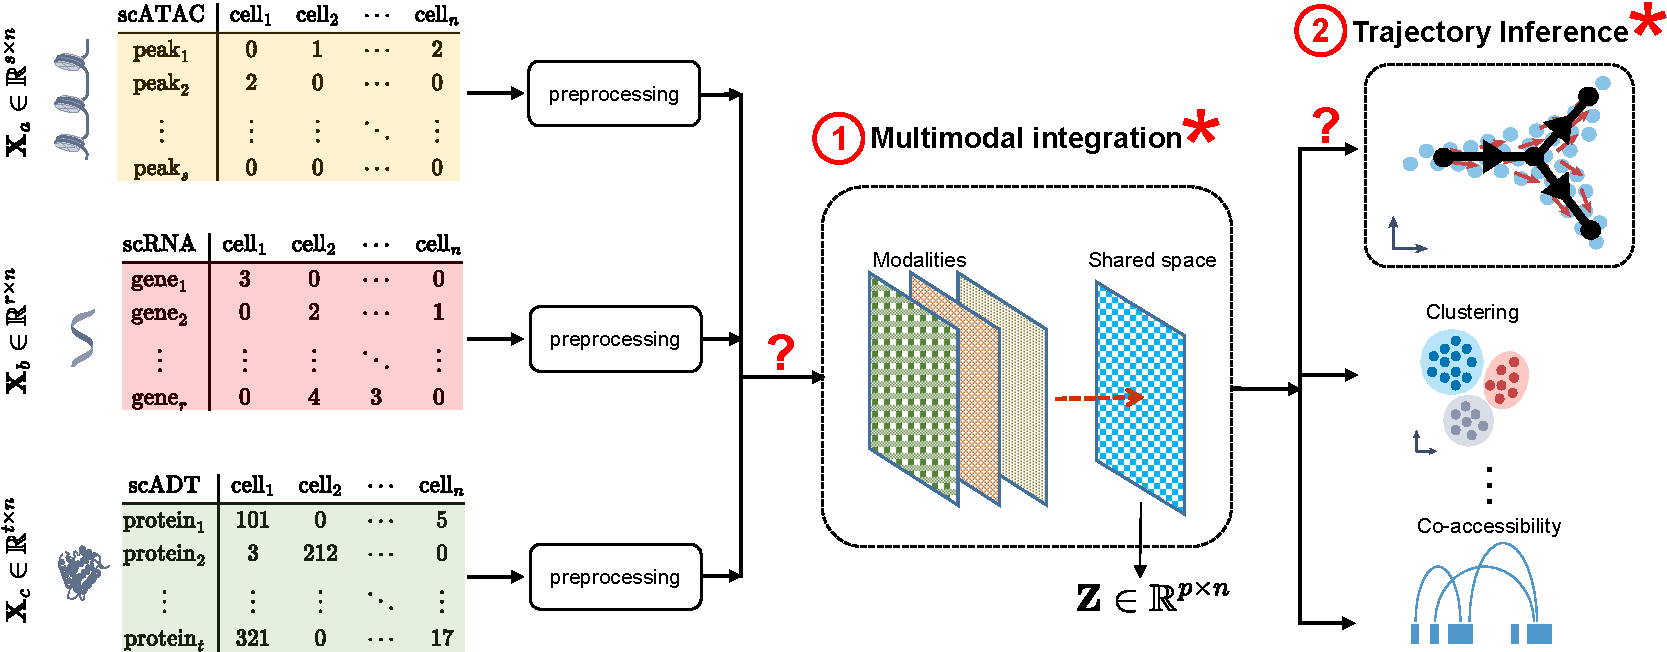
\includegraphics[width=0.95\textwidth]{workflow_multimodal/fig}
	\vspace{0.1cm}
	\caption[A common computational multimodal analysis workflow.]{A common computational workflow for single-cell multimodal dataset analysis involves several steps. Each count matrix from different modalities undergoes preprocessing, including quality checks and normalization. Subsequently, single-cell multimodal integration is performed to obtain a uniform latent space. Based on the latent space, downstream analyses can be conducted, such as clustering, trajectory inference, and visualization. Two key problems need to be addressed: \textcircled{\raisebox{-0.9pt}{1}} How to obtain a unified latent space for downstream analysis, and \textcircled{\raisebox{-0.9pt}{2}} Are there trajectory inference methods that can cooperate with multiple modalities?}
	\label{fig:workflow_multimodal}
\end{figure}

	%While many analyses developed for unimodal datasets can be adapted for multimodal data, establishing a consistent dimension reduction approach~(data integration) is advantageous for subsequent analyses.

	As illustrated in \fref{fig:workflow_multimodal}, following the preprocessing steps for each modality, the subsequent objective is to integrate these modalities to derive a consistent latent space. This unified latent space facilitates downstream analyses, including trajectory analysis, clustering, and visualization. It is crucial to emphasize the importance of batch correction, particularly when working with multiple batches of data, prior to integration.

	In addition to the downstream analysis for unimodal data, the incorpoartion of multiple modalities can enhance specific tasks performed in unimodal analysis, leading to more profound insights, such as achieving more accurate Gene Regulatory Networks~(GRN). For instance, scMega~\citep{li2023scmega} utilizes scRNA-seq and scATAC-seq data to infer GRN. And the integration of scRNA-seq and proteomic data proves valuable for a detailed examination of signaling networks~\citep{heumos2023best}.



% table of single cell trajectory inference methods

% a figure of single cell trajectory inference methods theory
\section{Discussion}
\label{background:Discussion}
In this chapter, we initially provided an overview of DNA structure and gene regulatory processes. Subsequently, we introduced the profiling techniques for single-cell transcriptome, epigenome, and proteome, including simultaneous profiling protocols. We then delved into the computational analyses associated with these modalities. Subsequently, we directed our focus towards computational analysis methods for single-cell multimodal data. We addressed the challenges posed by two critical analyses: single-cell multimodal integration and trajectory inference. We discussed the related work and outlined our objectives for tackling these tasks.
